\documentclass{article}
\usepackage[slovene]{babel}
\pdfpagewidth=8.5in
\pdfpageheight=11in
\usepackage{ijcai19}
\usepackage{listings}
% Use the postscript times font!
\usepackage{times}
\usepackage{soul}
\usepackage{url}
\usepackage[hidelinks]{hyperref}
\usepackage[utf8]{inputenc}
\usepackage[small]{caption}
\usepackage{graphicx}
\usepackage{amsmath}
\usepackage{multirow}
\usepackage{longtable}
\usepackage{geometry}
\usepackage{array}
\usepackage{booktabs}
\usepackage{makecell}

\urlstyle{same}

\title{Prva domača naloga}

\author{
Matej Klančar (63200136)
}

\begin{document}
\maketitle
\vspace{-1.5cm}
\section{Uvod}
To poročilo predstavlja rešitev prve domače naloge, 
ki se osredotoča na dva osrednja problema: učinkovito shranjevanje 
redkih matrik in iterativno reševanje linearnih sistemov.

V prvem delu je opisana implementacija podatkovnega tipa 
\texttt{RedkaMatrika} v jeziku Julia, vključno z osnovnimi operacijami, 
kot sta indeksiranje in množenje z vektorjem. V nadaljevanju je predstavljena 
implementacija metode SOR (Successive Over-Relaxation) za reševanje sistema 
$A\boldsymbol{x} = \boldsymbol{b}$.

Poročilo se zaključi z analizo, v kateri za testni primer poiščemo 
optimalni relaksacijski parameter $\omega$ in prikažemo njegov vpliv na hitrost 
konvergence.

\section{Implementacija}

V tem poglavju bomo podrobneje predstavili implementacijo podatkovnega 
tipa \texttt{RedkaMatrika} v programskem jeziku Julia. Cilj je bil ustvariti 
učinkovito predstavitev za matrike z velikim številom ničelnih elementov.

\subsection{Podatkovna struktura \texttt{RedkaMatrika}}

Osnova naše implementacije je podatkovna struktura \texttt{RedkaMatrika}. 
Struktura vsebuje dve polji:
\begin{itemize}
    \item \texttt{V}: Matrika, ki hrani vrednosti neničelnih elementov. Vsaka 
    vrstica v \texttt{V} ustreza enakoležni vrstici v redki matriki.
    \item \texttt{I}: Matrika, ki hrani stolpčne indekse neničelnih elementov. 
    Struktura te matrike je enaka matriki \texttt{V}.
\end{itemize}
Element na mestu \texttt{V[i, k]} hrani vrednost neničelnega elementa v 
\texttt{i}-ti vrstici redke matrike, njegov stolpčni indeks pa je shranjen 
na mestu \texttt{I[i, k]}. Mesta, ki še niso zasedena, imajo v matriki 
\texttt{I} vrednost 0.

\subsection{Indeksiranje}
Za smiselno uporabo našega tipa je bilo treba implementirati standardni 
vmesnik za indeksiranje, ki ga v Julii predstavljata funkciji \texttt{getindex} 
in \texttt{setindex!}.

\subsubsection{Pridobivanje elementov (\texttt{Base.getindex})}

Funkcija \texttt{getindex} omogoča branje vrednosti z običajno sintakso 
\texttt{T[i, j]}. Implementacija najprej poišče vrstico v matriki indeksov 
\texttt{T.I}, ki ustreza iskani vrstici \texttt{i}. Nato v tej vrstici s 
funkcijo \texttt{findfirst} poišče iskani stolpčni indeks \texttt{j}.

\begin{itemize}
    \item Če \texttt{findfirst} vrne \texttt{nothing}, stolpec \texttt{j} ni 
    med shranjenimi indeksi za vrstico \texttt{i}. Element je torej enak nič.
    \item Če \texttt{findfirst} vrne pozicijo \texttt{index}, funkcija na tej 
    isti poziciji v matriki vrednosti \texttt{T.V} poišče in vrne shranjeno 
    vrednost \texttt{T.V[i, index]}.
\end{itemize}

\subsubsection{Nastavljanje elementov (\texttt{Base.setindex!})}
Funkcija \texttt{setindex!} omogoča nastavljanje vrednosti s sintakso 
\texttt{T[i, j] = v}. Implementacija je kompleksnejša, saj mora obravnavati 
več primerov.

\begin{enumerate}
    \item \textbf{Spreminjanje obstoječega neničelnega elementa:} Najprej preverimo, ali na mestu \texttt{(i, j)} že obstaja neničelni element 
    (z uporabo naše funkcije \texttt{getindex}). Če obstaja, poiščemo 
    njegov indeks in posodobimo vrednost v matriki \texttt{V}.
    \item \textbf{Dodajanje novega neničelnega elementa:} Če element na 
    mestu \texttt{(i, j)} ne obstaja (je 0), moramo zanj poiskati prostor. 
    \begin{itemize}
        \item \textbf{Prosto mesto obstaja:} V \texttt{i}-ti vrstici matrike \texttt{I} poiščemo prvo prosto mesto, označeno z \texttt{0}. Na to mesto vpišemo nov stolpčni indeks \texttt{j}, na ustrezno mesto v matriki \texttt{V} pa vrednost \texttt{v}.
        \item \textbf{Ni prostega mesta:} Če so vsa mesta v vrstici že 
        zasedena, matriki \texttt{V} in \texttt{I} dinamično razširimo z 
        dodajanjem novega stolpca. Nato novo vrednost in indeks vpišemo na 
        novo vstavljeno mesto.
    \end{itemize}
\end{enumerate}

\subsection{Množenje z vektorjem}
Algoritem deluje po definiciji matričnega množenja. Ustvarimo nov ničelni vektor \texttt{b}. 
Nato z dvema gnezdenima zankama iterira čez vse elemente \texttt{(i, j)} 
navidezne polne matrike. V vsakem koraku 
izračuna produkt \texttt{T[i, j] * v[j]} in ga prištejemo \texttt{i}-ti 
komponenti rezultata \texttt{b[i]}.


\section{Reševanje linearnih sistemov z metodo SOR}

Za reševanje linearnih sistemov oblike $A\boldsymbol{x} = \boldsymbol{b}$, 
kjer je $A$ naša \texttt{RedkaMatrika}, smo implementirali iterativno 
metodo SOR. Ta je posebej primerna za velike, redke sisteme, saj 
iterativno izboljšuje približek rešitve.

\subsection{Algoritem metode SOR}
Metoda SOR posodobi vsako komponento vektorja rešitve 
$\boldsymbol{x}$ v koraku $k+1$ po formuli:
\begin{equation}
x_i^{(k+1)} = (1 - \omega) x_i^{(k)} + \frac{\omega}{A_{ii}} 
\left( b_i - \sum_{j<i} A_{ij}x_j^{(k+1)} - \sum_{j>i} A_{ij}x_j^{(k)} \right).
\label{eq:sor_short}
\end{equation}
Ključna značilnost metode je, da pri izračunu nove vrednosti $x_i^{(k+1)}$ 
takoj uporabi že posodobljene komponente iz iste iteracije (za $j<i$). 
Parameter $\omega$ (omega) uravnava hitrost konvergence.

\subsection{Implementacija}
Naša implementacija je sestavljena iz dveh glavnih delov:
\begin{enumerate}
    \item \textbf{Izvedba enega koraka iteracije:} Pomožna funkcija 
    \texttt{sor\_korak} izvede en sam prehod čez vse komponente vektorja 
    $\boldsymbol{x}$ v skladu s formulo~\eqref{eq:sor_short}. Za vsako 
    komponento $x_i$ izračuna vsoto produktov $A_{ij}x_j$ za $j \neq i$ in 
    nato posodobi vrednost $x_i$. Ker se vektor rešitve posodablja sproti 
    znotraj istega koraka, so pri izračunu za $x_i$ že uporabljene nove 
    vrednosti za vse $j<i$.

    \item \textbf{Glavna zanka in pogoj za ustavitev:} Glavna funkcija 
    \texttt{sor} zaporedno kliče \texttt{sor\_korak} in po vsaki iteraciji 
    preverja pogoj za ustavitev. Iteracija se ustavi, ko je neskončna norma 
    vektorja ostanka, $\|A\boldsymbol{x}^{(k)} - \boldsymbol{b}\|_\infty$, 
    manjša od podane tolerance \texttt{tol}. To v praksi pomeni, da se ustavi, 
    ko največja absolutna vrednost katerekoli komponente vektorja ostanka pade 
    pod tolerančno mejo.
\end{enumerate}

Funkcija sprejme matriko sistema $A$, vektor desnih strani 
$\boldsymbol{b}$, začetni približek $\boldsymbol{x_0}$, parameter $\omega$ in 
toleranco \texttt{tol}. V primeru uspešne konvergence vrne končni približek 
rešitve $\boldsymbol{x}$. Za preprečevanje neskončnega izvajanja v primeru 
nekonvergence je vgrajena tudi omejitev največjega števila iteracij.

\section{Analiza optimalnega parametra \(\omega\)}
Za metodo SOR je ključnega pomena pravilna izbira parametra $\omega$, 
saj ta neposredno vpliva na hitrost konvergence. 
Da bi poiskali optimalno vrednost za naš testni primer, smo 
izvedli numerično analizo. Metodo SOR smo pognali za različne 
vrednosti $\omega$ v intervalu $(0, 2)$ in zabeležili število 
iteracij, potrebnih za dosego tolerance $10^{-10}$.

\begin{figure}[h!]
    \centering
    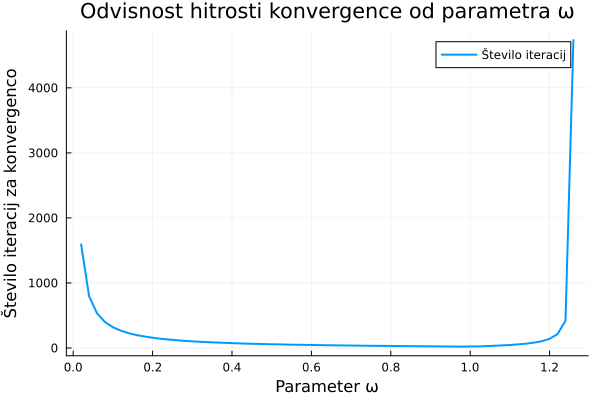
\includegraphics[width=0.9\textwidth]{sor_omega_konvergenca.png}
    \caption{Odvisnost števila iteracij od vrednosti parametra $\omega$.}
    \label{fig:sor_omega}
\end{figure}

Rezultati, prikazani na sliki \ref{fig:sor_omega}, kažejo jasno odvisnost
hitrosti konvergence od izbire $\omega$. Ugotovili smo, da je za 
obravnavani sistem optimalna vrednost parametra \textbf{$\omega = 0.98$}. 
Pri tej vrednosti je metoda konvergirala v \textbf{21 iteracijah}. Za $\omega$
večji ali enak 1.28 metoda ni konvergirala.
\end{document}

